
\chapter{Menu a tendina}

\section{Menu File}

Il menu file contiene i comandi per salvare la configurazione e aprire/chiudere la console.

\begin{figure}[H]
\centering
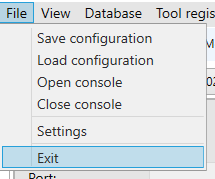
\includegraphics[width=0.3\textwidth]{../Img/Menu_File.PNG}
\caption{Menu File}
\end{figure}

\section{Menu View}

Nel menu view è possibile cambiare la lingua del programma così come visualizzare e
nascondere le colonne dei registri delle varie tab come si vede nell'immagine seguente:

\begin{figure}[H]
\centering
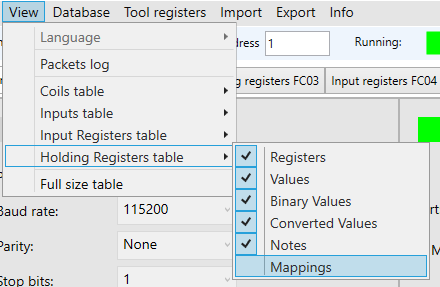
\includegraphics[width=0.6\textwidth]{../Img/Menu_View.PNG}
\caption{Menu View}
\end{figure}

\section{Menu Database}

Nel menu database è possibile creare/caricare un profilo e accedere al tool di import/export dei
profili. L'ultima voce del menu "Open temprate editor" apre la finestra di modifica dei template
personalizzati.

\begin{figure}[H]
\centering
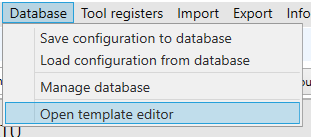
\includegraphics[width=0.45\textwidth]{../Img/Menu_Database.PNG}
\caption{Menu Database}
\end{figure}

\section{Menu Tools}

Nel menu tools è possibile aprire le finestre di comando per pilotare singoli bit/byte/word.

\begin{figure}[H]
\centering
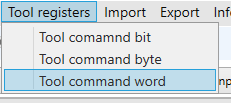
\includegraphics[width=0.32\textwidth]{../Img/Menu_Tools.PNG}
\caption{Menu Tools}
\end{figure}

\section{Menu Import}

Nel menu import è possibile inportare una tabella 
coils o holding registers esportata precedentemente
inviarla inviarla allo slave. Nel caso in cui i registri 
siano consecutivi è possibile scegliere se
inviarli singolarmente (write single coil/write single register) o in blocco 
(write multiple coils/write multiple registers).
E' possibile importare direttamente un file csv/json oppure
importare direttamente celle copiate (ctrl+c) da un foglio di calcolo
(clipboard).

\begin{figure}[H]
\centering
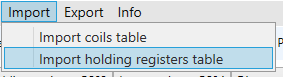
\includegraphics[width=0.4\textwidth]{../Img/Menu_Import.PNG}
\caption{Menu Import}
\end{figure}

\newpage
\section{Menu Export}

Nel menu export è possibile esportare le tabelle delle varie schede in formato csv.

\begin{figure}[H]
\centering
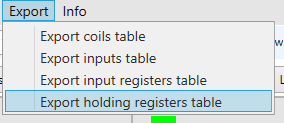
\includegraphics[width=0.4\textwidth]{../Img/Menu_Export.PNG}
\caption{Menu Export}
\end{figure}

\section{Menu Info}

Dal menu info è possibile aprire questa guida, visualizzare la licenza del programma e
data/numero di build.

\begin{figure}[H]
\centering
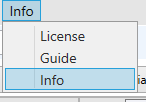
\includegraphics[width=0.25\textwidth]{../Img/Menu_Info.PNG}
\caption{Menu Info}
\end{figure}

Nella finestra info è possible leggere, oltre alla versione corrente, anche data e ora di build.

\begin{figure}[H]
\centering
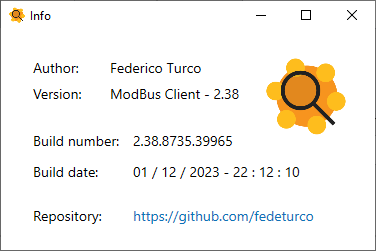
\includegraphics[width=0.5\textwidth]{../Img/Finestra_Info.PNG}
\caption{Finestra Info}
\end{figure}